\documentclass[hyperref={unicode=true}]{beamer}
\usepackage{multirow}
\usepackage{minted}
\usepackage{amsmath} % used for boldsymbol.
\renewcommand{\vec}[1]{\boldsymbol{#1}} % Uncomment for BOLD vectors.
\usepackage[slantfont,boldfont]{xeCJK}
\setCJKmainfont{SimSun}
\setCJKmonofont{FZFangSong-Z02}
\setCJKsansfont{SimHei}
\usetheme{Darmstadt}
\usecolortheme{beaver}
\usepackage{booktabs}
\usepackage{tikz}
\setbeamertemplate{theorems}[numbered]
\newtheorem{mytht}{\bf 定理}
\theoremstyle{definition}
\newtheorem{mydef}[]{\bf 定义}
\theoremstyle{proof}
\newtheorem{myprf}[]{\bf 证明}
\usepackage{ulem}
\usepackage[T1]{fontenc}
\usepackage{inconsolata}
\makeatletter
% there's no italic/slanted for Inconsolata
\@namedef{T1/zi4/m/it}{<->ssub*zi4/m/n}
\@namedef{T1/zi4/b/it}{<->ssub*zi4/b/n}
\@namedef{T1/zi4/bx/it}{<->ssub*zi4/b/n}
\@namedef{T1/zi4/m/sl}{<->ssub*zi4/m/n}
\@namedef{T1/zi4/b/sl}{<->ssub*zi4/b/n}
\@namedef{T1/zi4/bx/sl}{<->ssub*zi4/b/n}
\makeatother

\input zhwinfonts
\begin{document}
\setbeamertemplate{caption}[numbered]
\renewcommand\figurename{图}
\renewcommand\tablename{表}
\renewcommand\contentsname{\centering 目录}


%%------------------------------------------
\title{动态规划进阶(二)}
\subtitle{数位统计动态规划与状态压缩动态规划}
\author{马玉坤}
\institute{哈尔滨工业大学计算机科学与技术学院}
\date{2017年8月18日}
%%------------------------------------------

\begin{frame}\titlepage\end{frame}

\begin{frame}\tableofcontents\end{frame}

\section{数位统计动态规划}


\subsection{理论}
\begin{frame}\frametitle{数位统计动态规划}
  \begin{block}{一般形式}
    给定一个区间$[L,R]$,求在此区间内满足某个条件限制(特性)的数的个数或者加和。一般有多组询问。
  \end{block}
  \begin{exampleblock}{一般套路}
    \begin{enumerate}[<+->]
    \item 先将问题$[L,R]$转化为$[1,L-1]$和$[1,R]$的问题
    \item dp状态有两部分:
      \begin{enumerate}
      \item 跟枚举有关的部分:已枚举到的位数,以及前若干位数是不是已经到了上限(范围的限制)
      \item 跟特性有关的部分:已枚举的位上的数已经到达的状态(特性的限制)
      \end{enumerate}
    \end{enumerate}
  \end{exampleblock}
\end{frame}
\begin{frame}\frametitle{数位统计动态规划 (Cont'd)}
  \begin{alertblock}{对解题的忠告}
    \begin{enumerate}[<+->]
    \item 数位DP较容易对拍,可以本地测试,减少WA
    \item 耐心,细心
    \item 重构/重写
    \end{enumerate}
  \end{alertblock}
\end{frame}

\subsection{题目}
\subsubsection{Find a car}
\begin{frame}{Find a car}\framesubtitle{Codeforces Round \#415 (Div. 1) C}
  \begin{block}{题目}
    给定一个无穷大的矩阵,其中第i行第j列的元素$mat(i,j)$为最小的不在集合$\{mat(1,j),mat(2,j),\ldots,mat(i-1,j), mat(i,1), mat(i,2), \ldots,mat(i,j-1)\}$中出现过的正整数。
    \begin{minipage}{0.45\linewidth}
      \begin{figure}
        \centering
        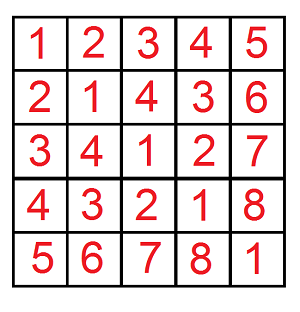
\includegraphics[width=1.2in]{figures/upper5.png}
        \caption{矩阵左上角的5个元素}\label{fig:upper5}
      \end{figure}
    \end{minipage}
    \begin{minipage}{0.45\linewidth}
      然后会有$Q(\leq 10^4)$个询问,每个询问给定$x_1,y_1,x_2,y_2,k$,回答子矩阵$(x_1,y_1)-(x_2,y_2)$内所有小于小于等于$k$的数的和。$x_1,y_1,x_2,y_2\leq 10^9$且$k\leq2\times 10^9$。
    \end{minipage}
  \end{block}
\end{frame}

\begin{frame}{Find a car (Cont'd)}\framesubtitle{Codeforces Round \#415 (Div. 1) C}
  \begin{alertblock}{第一个问题}
    第i行第j列,即$mat(i,j)$该怎么求?能不能用一个简单的式子来表示?\\
    \pause{}先把矩阵里的每个元素都减1,行数和列数从1开始变为从0开始。\\
    \pause{}此时可转化为两堆石子(分别为$i$和$j$),做NIM游戏。$mat(i,j)=\text{各个子状态的SG函数}=i \oplus j$ ($\oplus$为异或)。对于原矩阵就有$mat(i,j)=(i-1)\oplus (j-1) + 1$。\\
    {\bf 不懂原理也没关系,今天我们的重点不在这。}
  \end{alertblock}
\end{frame}

\begin{frame}{Find a car (Cont'd)}\framesubtitle{Codeforces Round \#415 (Div. 1) C}
  \begin{block}{异或}
    \begin{figure}
      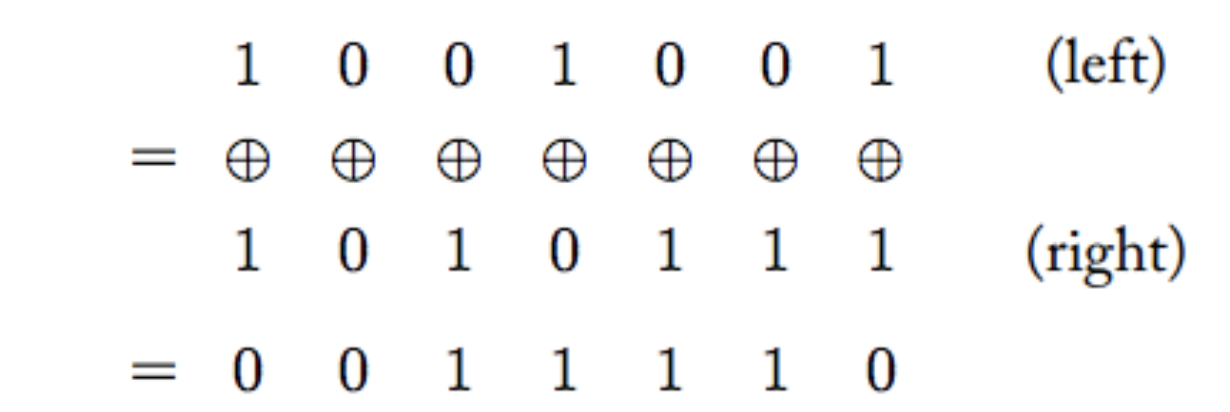
\includegraphics[width=2.3in]{figures/xor.png}
      \caption{异或}\label{fig:xor}
    \end{figure}
  \end{block}
\end{frame}

\begin{frame}{Find a car (Cont'd)}\framesubtitle{Codeforces Round \#415 (Div. 1) C}
  \begin{block}{二维前缀和}
    设$sum(x,y)=\sum_{i=1}^x \sum_{j=1}^j a(i,j)$,那么我们有
    \begin{align}
      &\sum_{i=x_1}^{x_2} \sum_{j=y_1}^{y_2} a(i,j)\\
      =&sum(x_2,y_2)-sum(x_1-1,y_2)\\
      &-sum(x_2,y_1-1)+sum(x_1-1,y_1-1)
      \end{align}
  \end{block}
\end{frame}

\begin{frame}{Find a car (Cont'd)}\framesubtitle{Codeforces Round \#415 (Div. 1) C}
  \begin{exampleblock}{数位DP}
    问题转化成求$\sum_{i=1}^{x}\sum_{j=1}^{y}[i\oplus j\leq k](i \oplus j)$\\
    设$f(di,dx,dy,dk)$为这个状态下的数字个数,$g(di,dx,dy,dk)$为数字和。其中$di$表示从最高位开始已枚举到的位数,$dx,dy$分别表示已枚举的$x$与$y$的前缀是否到达上限,$dk$表示已枚举的$x$和$y$的前缀的异或是否达到$k$的上限。\\
    详见代码。
  \end{exampleblock}
\end{frame}

\begin{frame}{Find a car (Cont'd)}\framesubtitle{Codeforces Round \#415 (Div. 1) C}
  \begin{exampleblock}{数位DP (Cont'd)}
    为什么这样设计状态?举个例子。\\
    比如$x=1010,y=0101,k=1110$,枚举完了高三位,此时已枚举的$x'=101$,$y'=010$,且它们的异或值$k'=111$,这时候的状态应该是$f(0,1,1,1)$(枚举到第0位,且$x,y,k$前缀都达到限制)。\\
    那么我们枚举低位的时候就不能随便枚举$x$和$y$,否则会超出$x$和$y$的限制。同时,我们还要注意已枚举的前缀是否达到$k$的上限,如果达到了$k$的上限,同样不能随便枚举$x$和$y$。枚举第0位时,我们实际上x只能取0,y只能取0或1,但y不能取1,因为这时候$x\oplus y=1111$,超出了范围。
  \end{exampleblock}
\end{frame}

\begin{frame}{Find a car (Cont'd)}\framesubtitle{Codeforces Round \#415 (Div. 1) C}
  \begin{exampleblock}{总结}
    四个状态中前三个状态(位数,x前缀,y前缀)都是关于枚举的范围的,而第四个状态可以理解成枚举的范围,也可以理解成数的特性。在这里我们使用了布尔变量,表示前缀是否达到上限,从而使得我们枚举后面的位时知道是否需要注意范围的限制。
  \end{exampleblock}
\end{frame}

\subsubsection{两种dp数组求解的写法}
\begin{frame}[fragile]{递推求动态规划}
  \begin{minted}[fontfamily=zi4]{C++}
for (int i = 0; i < n; i++) {
  for (int j = volume[i]; j <= capacity; j++) {
    dp[i][j] = max(dp[i-1][j],
                   dp[i-1][j-volume[i]] + value[i]);
  }
}
  \end{minted}
\end{frame}

\begin{frame}[fragile]{递归求动态规划(记忆化搜索)}
  \begin{minted}[fontfamily=zi4]{C++}
int dfs(int i, int j) {
  if (i == 0) {
    return 0;
  }
  if (vis[i][j]) {
    return dp[i][j];
  }
  vis[i][j] = 1;
  return dp[i][j] = max(dfs(i-1, j-1),
                        dfs(i-1, j-volume[i]) + value[i]);
}
  \end{minted}
\end{frame}
\begin{frame}{两种方法的比较}
  \begin{itemize}[<+->]
  \item 递推的优势
    \begin{enumerate}
    \item 常数小
    \item 不需递归,不怕爆栈
    \end{enumerate}
  \item 递归的优势
    \begin{enumerate}
    \item 对有效状态数较少的问题可大大提高效率,避免无效状态的搜索
    \item 实现简单,更符合人类思维
    \end{enumerate}
  \end{itemize}
\end{frame}


\subsubsection{K-wolf Number}
\begin{frame}{K-wolf Number (Cont'd)}\framesubtitle{2016 Multi-University Training Contest 5 07}
  \begin{block}{问题}
    K-wolf数字定义为:十进制表示下,任意相邻的k位数字都各不相同。\\
    给定$L,R,K$,求区间$[L,R]$内的K-wolf数字的个数。\\
    $L,R\leq10^{18};K\leq5$
  \end{block}
\end{frame}

\begin{frame}{K-wolf Number (Cont'd)}\framesubtitle{2016 Multi-University Training Contest 5 07}
  \begin{exampleblock}{解法}
    转化为$1,\ldots,n$的K-wolf数个数的问题。\\
    设$dp(i,j,k)$表示从最高位枚举到第i位,j表示已枚举的位有没有达到n的上限,k存的是已枚举的位中后k-1位的值。这样我们就能知道。\\
  \end{exampleblock}
\end{frame}

\begin{frame}{K-wolf Number (Cont'd)}\framesubtitle{2016 Multi-University Training Contest 5 07}
  \begin{exampleblock}{解法 (Cont'd)}
    注意到一个问题:刚才的题目 (Find a car)中,我们实际上将所有数都加上了前导零,补成了31位。然而在这个题目中,如果我们仍然这么操作,从第8位开始枚举,补上前导零,把所有数都变成18位数,那么像29这样的数就会变成000000000000000029,不符合K-wolf数的定义 (有连续的0),所以我们不能算上前导零。\\
    \pause{}一种方案是:在dp状态中,加入一维指示之前枚举的位是否全是0。\\
    另一种方案是:手动枚举数的位数以及最高位的数字,然后剩下再dp。\\
    \pause{}具体实现见文件k-wolf\_1.cpp与k-wolf\_2.cpp。
  \end{exampleblock}
\end{frame}

\subsubsection{淘金}
\begin{frame}{淘金}\framesubtitle{SDOI 2013 Round 1 Day 2 Problem 3}
  \begin{block}{题目}
    初始时,在$1 \leq x \leq n, 1 \leq y \leq n$上的每个点上,都有一块金子。在一阵风过后,$(x,y)$位置上的金子会到$(f(x),f(y))$位置上,其中$f(x)$等于$x$各个位上的数字乘积。\\
    这阵风刮过之后,小Z希望依次走到k个点上进行金子的收集。请最大化收集到的金子总数。结果对$10^9+7$取模。\\
    $n\leq 10^{12};k \leq \min(10^5, n^2)$
  \end{block}
\end{frame}

\begin{frame}{淘金 (Cont'd)}\framesubtitle{SDOI 2013 Round 1 Day 2 Problem 3}
  \begin{alertblock}{第一个问题}
    最后有多少个金子落到了$(x,y)$坐标上?\\
    \pause{}\[(\sum_{i=1}^n[f(i)=x])\times(\sum_{j=1}^n[f(j)=y])\]
    所以为了简化,把x与y坐标分开考虑。
  \end{alertblock}
\end{frame}

\begin{frame}{淘金 (Cont'd)}\framesubtitle{SDOI 2013 Round 1 Day 2 Problem 3}
  \begin{alertblock}{第二个问题}
    只考虑一维的话,什么样的坐标上会有金子?\\
    \pause{}质因子只包括$2,3,5,7$(当然也可以不包括)。\\
    \[\log_2{10^{12}} \times \log_3{10^{12}} \times \log_5{10^{12}} \times \log_7{10^{12}} \approx 244411 \]
    实际上,有金子的坐标数没那么$10^{12}$多。
  \end{alertblock}
\end{frame}

\begin{frame}{淘金 (Cont'd)}\framesubtitle{SDOI 2013 Round 1 Day 2 Problem 3}
  \begin{exampleblock}{数位DP}
    设$dp(i,l,c_2,c_3,c_5,c_7)$。$i$表示枚举到的位数,$l$表示已枚举的位是否达到n的上限,$c_2,c_3,c_5,c_7$分别表示已枚举的位上的数相乘得到的乘积中$2,3,5,7$四种质因子的数目。
  \end{exampleblock}
\end{frame}

\begin{frame}{淘金 (Cont'd)}\framesubtitle{SDOI 2013 Round 1 Day 2 Problem 3}
  \begin{exampleblock}{其实还有一个问题}
    给定序列$a_1,a_2,\ldots ,a_n$(已经从大到小排好序),在矩阵$M$中找到前m大的值的和。其中$M_{i,j}=a[i]\times a[j]$。\\
    \pause{}最大值可能是$a_1\times a_1,a_2 \times a_1, \ldots, a_n \times a_1$,然后呢?(显然$a_1 \times a_1$最大。)\\
    次大值可能是$a_1 \times a_2,a_2\times a_1, a_3 \times a_1,\ldots,a_n \times a_1$。然后呢?(假设$a_2 \times a_1$最大。)\\
    第3大值可能是$a_1 \times a_2, a_2 \times a_2, a_3 \times a_1, a_n \times a_1$。\\
    维护矩阵每一行从左往右第一个没遍历的元素,然后放入最大堆中,每次从堆顶中取出$x$,此时$x$所在的行的第一个没遍历的元素变成了$x$右边的数,把$x$弹出,并把$x$右边的数加入堆中。重复m次。时间复杂度$O((m+n) \log{n})$。\\
    实际上还可以优化到$O(m \log{n})$。
  \end{exampleblock}
\end{frame}

\section{状态压缩动态规划}

\subsection{原理}
\begin{frame}{使用二进制数进行状态压缩}
  \begin{block}{使用二进制数表示状态的动机}
    \begin{itemize}
    \item 很多问题中,每个元素都有两种状态(在集合中,不在集合中;被占据,没被占据)
    \item 计算机使用二进制存储数据,使用原生的数字运算便可实现很多集合运算
    \end{itemize}
  \end{block}
\end{frame}

\begin{frame}{使用二进制数进行状态压缩 (Cont'd)}
  \begin{exampleblock}{使用二进制数表示状态的方法}
    \begin{enumerate}
    \item $\&$: “与”运算,集合求交
    \item $|$: “或”运算,集合求并
    \item $\wedge$: “异或”运算,集合对称差 ($(A-B) \cup (B-A)$),一般用作求补集 (也就是左操作数表示的集合包含右操作数表示的集合时使用)
    \item $<<$: “左移”运算,$x<<d$,将x在二进制下的每一位向左移动d位,最右边用0填充
    \item $>>$: “右移”操作,$x>>d$,将x在二进制下的每一位向右移动d位,最左边用0填充(只考虑正数或无符号数)
    \end{enumerate}
    例子:$((S>>5)\&1)$——获取S状态下第5个元素的状态。
  \end{exampleblock}
\end{frame}
\begin{frame}{其他方法}
  \begin{exampleblock}{视题目而定}
    有些题目中元素状态有若干种,例如连通性状态压缩动态规划中,插头的种类数就决定了每个元素的状态数目。\\
    3进制、4进制、阶乘表示都有可能。
  \end{exampleblock}
\end{frame}

\subsection{题目}
\subsubsection{Stabilization}
\begin{frame}{Stabilization}\framesubtitle{2016 Multi-University Training Contest 6 06}
  \begin{block}{题目}
    给定序列$a_1,a_2,\ldots,a_n$,求一个$x$,使得
    \[\sum_{i=1}^{n-1}{|(a_{i+1} \oplus x) -  (a_{i} \oplus x)|}\]
    最小。\\
    $n\leq 10^5;a_i < 2^{20}$
  \end{block}
\end{frame}

\begin{frame}{Stabilization (Cont'd)}\framesubtitle{2016 Multi-University Training Contest 6 06}
  \begin{alertblock}{第一个问题}
    异或$x$之后,相邻的数的大小关系会改变,怎么处理?\\
    \pause{}因为异或的是同一个数$x$。所以两个数不同的二进制位异或之后仍然不同,相同的二进制位异或之后仍然相同。\\
    \pause{}我们只需要看两个相邻的数的二进制表示中最高的不同的位,就可以知道相邻的两个数谁比谁大,谁减谁等于差的绝对值。
  \end{alertblock}
\end{frame}

\begin{frame}{Stabilization (Cont'd)}\framesubtitle{2016 Multi-University Training Contest 6 06}
  \begin{exampleblock}{解法}
    设$S_i=\{j|a_j\text{与}a_{j+1}\text{二进制表示中最高不同的位为}i\}$。我们可以设
    \begin{align}
      dp(x, i)&=\sum_{j\in S_i}{|(a_j\oplus x)-(a_{j+1} \oplus x)|}\\
      f(i)&=|S_i|\\
      g(i,k)&=\sum_{j \in S_i}[a_j\text{和}a_{j+1}\text{第}k\text{位分别为0和1}]\\
      h(i,k)&=\sum_{j \in S_i}[a_j\text{和}a_{j+1}\text{第}k\text{位分别为1和0}]
    \end{align}
  \end{exampleblock}
\end{frame}

\begin{frame}{Stabilization (Cont'd)}\framesubtitle{2016 Multi-University Training Contest 6 06}
  \begin{exampleblock}{解法 (Cont'd)}
    设$x$的二进制表示中最高的为 1 的位为第$highbit(x)$位。设$y=x\oplus2^{highbit(x)}$,此时假设我们算完了 $dp(y, 0 \ldots 19)$,怎么算$dp(x,0 \ldots 19)$呢?\\
    \pause{}$dp(x, 0 \ldots highbit(x)-1) = dp(y, 0 \ldots highbit(x)-1)$(这部分没有影响)\\
    \pause{}$dp(x, highbit(x)) = 2^{highbit(x)+1} \times f(highbit(x)) - dp(y, highbit(x))$(原来是$i-j$,因为最高不同的位取反,现在变成了$2^{highbit(x)+1}+j-i=2^{highbit(x)+1}-(i-j)$)\\
    \pause{}\begin{minipage}{0.45\linewidth}
      \begin{figure}
        \begin{center}
          $i$: 0 {\bf\uline{1}} 0 1 1 1 0\\
          $j$: 0 {\bf\uline{0}} 0 1 0 0 1
        \end{center}
        \caption{最高位取反前}
      \end{figure}
    \end{minipage}
    \begin{minipage}{0.45\linewidth}
      \begin{figure}
        \begin{center}
          $i$: 0 {\bf\uline{0}} 0 1 1 1 0\\
          $j$: 0 {\bf\uline{1}} 0 1 0 0 1
        \end{center}
        \caption{最高位取反后}
      \end{figure}
    \end{minipage}
  \end{exampleblock}
\end{frame}

\begin{frame}{Stabilization (Cont'd)}\framesubtitle{2016 Multi-University Training Contest 6 06}
  \begin{exampleblock}{解法 (Cont'd)}
    那$dp(x, highbit(x)+1 \ldots 19)$呢?留作练习题。\\
    注意:不要忘了用$g(i,k)$和$h(i,k)$。
  \end{exampleblock}
  \begin{block}{启示}
    需要预处理的东西都不是一下子就能想到的,需要在实际进行计算的尝试时才能发现。
  \end{block}
\end{frame}

\subsubsection{炮兵阵地}
\begin{frame}{炮兵阵地}\framesubtitle{NOI 2001}
  \begin{block}{问题}
    给定一个$n \times m$的网格图,需要在其上部署炮兵部队,网格图上的每个网格可能是平原(可以部署部队),或者是山地(不可以部署部队)。\\
    \begin{minipage}{0.45\linewidth}
      问最多能部署多少支炮兵部队,使任意两个部队不在对方的攻击范围,炮兵的攻击范围见图\ref{fig:attack}。\\
      $n \leq 100; m \leq 10$
    \end{minipage}
    \begin{minipage}{0.45\linewidth}
      \begin{figure}
        \centering
        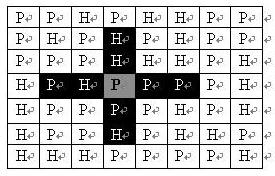
\includegraphics[width=1.4in]{figures/attack.png}
        \caption{炮兵部队攻击范围}\label{fig:attack}
      \end{figure}
    \end{minipage}
  \end{block}
\end{frame}

\begin{frame}{炮兵阵地 (Cont'd)}\framesubtitle{NOI 2001}
  \begin{exampleblock}{解法}
    按行转移做状态压缩动态规划。\\
    由于上下攻击范围是相互的,所以我们只需要让上面的部队不要打到下面就可以。\\
    设$dp(i,S)$表示第1行到第i行已经确定,且第i行的状态为$S$的方案数。S实际上可以用3进制数来表示。
    \begin{itemize}
    \item S的第j位为0,意味着$(i,j)$与$(i-1,j)$都没有放部队,此时$(i+1,j)$可以放部队
    \item S的第j位为1,意味着$(i-1,j)$放了部队,此时$(i+1,j)$不可以放部队
    \item S的第j位为2,意味着$(i,j)$放了部队,此时$(i+1,j)$也不可以放部队
    \end{itemize}
  \end{exampleblock}
\end{frame}

\begin{frame}{炮兵阵地 (Cont'd)}\framesubtitle{NOI 2001}
  \begin{exampleblock}{解法 (Cont'd)}
    有了第i行的状态的表示,我们就能知道第i+1行怎样枚举决策了,也就是说这一行放几支部队,分别放到哪。\\
    \pause{}第i行一共有$3^{10}$种状态,对于每个状态,第i+1行都有$2^{10}$个决策(每个格子放或者不放)。\\
    然而,事实上,有效的状态数并没有那么多,可以预处理一下有用的状态,加一些剪枝。比如,同一行不可能放两个相邻的炮兵部队(隔一个格子也不行)。
  \end{exampleblock}
\end{frame}

\subsubsection{多米诺骨牌覆盖问题}
\begin{frame}{多米诺骨牌覆盖问题}
  \begin{block}{问题}
    多米诺骨牌的大小为$1\times 2$,现在你要用多米诺骨牌去覆盖$n\times m$大小的方格图。使得方格图中的每个方格被且仅被一个多米诺骨牌的一格覆盖。\\
    \begin{minipage}{0.45\linewidth}
      问一共有多少覆盖方案?\\
      $n \times m \leq 256$
    \end{minipage}
    \begin{minipage}{0.45\linewidth}
      \begin{figure}
        \centering
        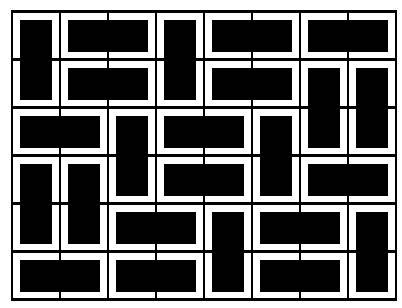
\includegraphics[width=1.4in]{figures/domino.png}
        \caption{$6\times 8$网格图的多米诺骨牌覆盖}
      \end{figure}
    \end{minipage}
  \end{block}
\end{frame}

\tikzset{global scale/.style={
    scale=#1,
    every node/.append style={scale=#1}
  }
}
\begin{frame}{多米诺骨牌覆盖问题 (Cont'd)}
  \begin{alertblock}{初步分析}
    $n \times m \leq 256$的意思是说$\min{(n,m)} \leq 16$,不失一般性,我们设$m\leq n$。(n为行数)\\
    这样每行的格子数不多($\leq 16$)。\\
    但不像上一个题里,我们一行一行地决策,这次我们一格一格地决策。
  \end{alertblock}
\end{frame}

\begin{frame}[fragile]{多米诺骨牌覆盖问题 (Cont'd)}
  \begin{exampleblock}{解法}
    \begin{minipage}{0.4\linewidth}
      \begin{figure}
        \centering
        \begin{tikzpicture}[global scale=1.5]

          \draw[thick] (0, 0.5) -- (1, 0.5);
          \draw[thick, red] (1, 0.5) -- (2.5, 0.5);
          \draw[thick, red] (0, 0) -- (1, 0);
          \draw[thick] (1, 1) -- (2.5, 1);
          \draw[thick] (0, 0) -- (0, 0.5);
          \draw[thick] (0.5, 0) -- (0.5, 0.5);
          \draw[thick, red] (1.0, 0) -- (1.0, 0.5);
          \draw[thick] (1.0, 0.5) -- (1.0, 1.0);
          \draw[thick] (1.5, 0.5) -- (1.5, 1.0);
          \draw[thick] (2.0, 0.5) -- (2.0, 1.0);
          \draw[thick] (2.5, 0.5) -- (2.5, 1.0);

          \draw[dotted] (1, 0) -- (1.5, 0);
          \draw[dotted] (1.5, 0) -- (1.5, 0.5);

          \draw (1, 0) node[anchor=south west]{{\scriptsize $i,j$}}
          (0, 0) node[anchor=south west]{{\scriptsize $1$}}
          (0.5, 0) node[anchor=south west]{{\scriptsize $0$}}
          (1.0, 0.5) node[anchor=south west]{{\scriptsize $0$}}
          (1.5, 0.5) node[anchor=south west]{{\scriptsize $1$}}
          (2.0, 0.5) node[anchor=south west]{{\scriptsize $0$}};

        \end{tikzpicture}
        \caption{轮廓线示意图(这图画起来好麻烦的)}
      \end{figure}
    \end{minipage}
    \begin{minipage}{0.58\linewidth}
      设$dp(i,j,S)$表示轮廓线状态为$S$时的方案数。$S$可以用一个二进制数表示,因为轮廓线上第$j$列的格子要么
      \begin{itemize}
      \item 0:没被覆盖
      \item 1:被覆盖了
      \end{itemize}
      \pause{}那么决策有哪几种呢?
      \begin{itemize}
      \item 放一个横着的骨牌(主动决策)
      \item 放一个竖着的骨牌(被动决策,要看上一行同列的方格有没有被覆盖)
      \end{itemize}
    \end{minipage}
  \end{exampleblock}
\end{frame}

\begin{frame}[fragile]{多米诺骨牌覆盖问题 (Cont'd)}
  \begin{exampleblock}{解法 (Cont'd)}
    代码写起来很简单。
    \begin{minted}[fontsize=\scriptsize, frame=lines, gobble=6, fontfamily=tt]{C++}
      #define _1(i, j) (((i)>>(j))&1)
      for (int i = 0; i < n; i++) {
        for (int j = 0; j < m; j++) {
          swap(cur, lst);
          dp[cur].clear();
          for (auto it = dp[lst].begin(); it != dp[lst].end(); ++it) {
            int s = it->first,
            v = it->second;
            if (j && !_1(s, j) && _1(s, j - 1)) {
              addMod(dp[cur][s ^ (1<<(j-1))], v);
            }
            addMod(dp[cur][s ^ (1<<j)], v);
          }
        }
        addMod(f[i][m], dp[cur].count(0)?dp[cur][0]:0);
      }

    \end{minted}
  \end{exampleblock}
\end{frame}

\end{document}
